%%%%%%%%%%%%%%% Page Setup %%%%%%%%%%%%%%%

\documentclass{beamer}
\usepackage[framemethod=tikz]{mdframed}
\setlength\parindent{0pt}
\setlength{\parskip}{\baselineskip}%
\usepackage{graphicx}
\usepackage{tgadventor}
%\renewcommand*\familydefault{\sfdefault}
\usepackage[T1]{fontenc}
\usepackage{fontspec}
\usefonttheme{professionalfonts} % using non standard fonts for beamer
\usefonttheme{serif} % default family is serif
\usetheme{Pittsburgh}
\usepackage{gradient-text}
\setbeamerfont{title}{size=\bfseries\huge}
%%%%%%%%%%%%%%% Math Stuff %%%%%%%%%%%%%%%

\usepackage{amsmath}
\usepackage{amssymb}
\usepackage{tikz}
\usepackage{tikz-cd}
\usepackage{tkz-euclide}
\usepackage{pgf-pie}
\usepackage{cancel}

%%%%%%%%%%%%%%% Quotation Stuff %%%%%%%%%%%%%%%

\usepackage[english]{babel}
\usepackage[autostyle]{csquotes}

%%%%%%%%%%%%%%% Color %%%%%%%%%%%%%%%

\definecolor{p}{rgb}{0.9118, 0.4961, 0.6804}
\definecolor{p1}{rgb}{1, 0.92, 0.963}
\definecolor{g}{rgb}{0.023, 0.477, 0.219}
\definecolor{g1}{rgb}{0.03, 0.75, 0.20}
\definecolor{g2}{rgb}{0.95, 1, 0.95}
\definecolor{b}{rgb}{0.02, 0.02, 0.02}

%%%%%%%%%%%%%%% Link Setup %%%%%%%%%%%%%%%

\usepackage{hyperref}
\hypersetup{colorlinks=true, linkcolor=g, filecolor=g, urlcolor=g,}

%%%%%%%%%%%%%%% Box %%%%%%%%%%%%%%%

\newmdenv[innerlinewidth=2pt, roundcorner=4pt,linecolor=g1,innerleftmargin=20pt,
innerrightmargin=20pt,innertopmargin=20pt,innerbottommargin=20pt,backgroundcolor = g2]{mybox}


%%%%%%%%%%%%%%% Bug Fix Adjustments %%%%%%%%%%%%%%%

\setlength{\headheight}{14pt}
\setlength{\footskip}{55pt}

%%%%%%%%%%%%%%% Index %%%%%%%%%%%%%%%

\usepackage{makeidx}
\makeindex

%%%%%%%%%%%%%%% Custom Commands %%%%%%%%%%%%%%%

\def\greenlozenge{\mathbin{\color{g}\blacklozenge}}

\newcommand{\emphasis}[1]{\underline{\textbf{#1}} }
\newcommand{\vocab}[1]{\underline{\textbf{\textcolor{red}{#1}}}}


%%%%%%%%%%%%%%% Math Operators %%%%%%%%%%%%%%%
\DeclareMathOperator{\A}{\mathbb{A}}
\DeclareMathOperator{\Aut}{Aut}
\DeclareMathOperator{\C}{\mathbb{C}}
\DeclareMathOperator{\characteristic}{char}
\DeclareMathOperator{\cod}{cod}
\DeclareMathOperator{\dom}{dom}
\DeclareMathOperator{\Fix}{Fix}
\DeclareMathOperator{\Frac}{Frac}
\DeclareMathOperator{\Free}{Free}
\DeclareMathOperator{\id}{id}
\DeclareMathOperator{\Ima}{Im}
\DeclareMathOperator{\Mor}{Mor}
\DeclareMathOperator{\N}{\mathbb{N}}
\DeclareMathOperator{\Obj}{Obj}
\DeclareMathOperator{\Q}{\mathbb{Q}}
\DeclareMathOperator{\R}{\mathbb{R}}
\DeclareMathOperator{\Res}{Res}
\DeclareMathOperator{\Stab}{Stab}
\DeclareMathOperator{\Span}{span}
\DeclareMathOperator{\Spec}{Spec}
\DeclareMathOperator{\Z}{\mathbb{Z}}
\DeclareMathOperator{\trdeg}{trdeg}
%%%%%%%%%%%%%%% Title %%%%%%%%%%%%%%%
\setbeamercolor{frametitle}{fg=g1,bg=g2}
\setbeamercolor{definition}{fg=g1,bg=g2}


\begin{document}

    \begin{frame}
        \begin{center}
            {\bfseries\huge\gradientRGB{Transcendental Numbers}{20,220,100}{50,200,200}} \par
        Vincent Lin \par
        \today
        \end{center}
    \end{frame}


    \begin{frame}
        \frametitle{Introduction}
    \begin{mybox}
        \textbf{Definition:} An \vocab{algebraic number} is $\alpha \in \C$, which is the root of a nonzero polynomial in $\Q[x]$ (or $\Z[x]$). We denote the set of algebraic numbers $\A$ or $\bar{\Q}$. Otherwise, it is \vocab{transcendental}.
    \end{mybox}
    \end{frame}

   
    \begin{frame}
        \frametitle{Examples of Algebraic Numbers}
        \[\frac{p}{q} \in \Q\]
        It is the root of $x - \frac{p}{q}$. Therefore, we can deduce that $\Q \subseteq \A$.
        $i$ is the root of $x^2 + 1$.
    \end{frame}

  
    \begin{frame}
        \frametitle{Examples of Transcendental Numbers}
        \begin{center}
            Do transcendental numbers even exist? Are there numbers which are not algebraic? 
        \end{center}
    \end{frame}

    \begin{frame}
        \frametitle{Existence of Transcendental Numbers}
        \begin{center}
            \begin{mybox}
                \textbf{Theorem:} Yes.
            \end{mybox}

            Why? $\C$ is uncountable, $\A$ is countable. Therefore, there are elements in $\C$ not in $\A$. Likewise, since $\R$ is uncountable, there are real transcendental numbers as well.
        \end{center}
    \end{frame}
    \begin{frame}
        \frametitle{Countability of Algebraic Numbers}
        \begin{center}
            $\A$ is countable. Let $p(x) = a_{n}x^{n} + \cdots + a_0 \in \Z[x]$ and let the index of $p$ be $\vert a_n \vert + \cdots + \vert a_0 \vert + n$. For each $i > 0$, list all $p$ with index $i$. Then, list their roots. 
        \end{center}
    \end{frame}

    \begin{frame}
        \frametitle{Countability of Algebraic Numbers}
            \[\text{index = 1: None} \]
            No new roots. \\
            \noindent\makebox[\linewidth]{\rule{\paperwidth}{0.4pt}}
            \[\text{index = 2: } \pm x \]
            New roots: $\{0\}$ \\
            \noindent\makebox[\linewidth]{\rule{\paperwidth}{0.4pt}}
            \[\text{index = 3: } \pm x^2, \pm x \pm 1, \pm 2x\]
            New roots: $\{\pm 1\}$
            \noindent\makebox[\linewidth]{\rule{\paperwidth}{0.4pt}}
            \[\ldots\]

    \end{frame}

    \begin{frame}
        \frametitle{Countability of Algebraic Numbers}
        \begin{center}
    Eventually, every algebraic number will be listed because it is the root of a polynomial $\Z[x]$ with finite index. Thus, $\A$ is countable and has measure $0$. However, it is dense in $\C$.\par
    \[\greenlozenge\]
    \end{center}
    \end{frame}

    \begin{frame}
        \frametitle{First Transcendental Number}
        \begin{center}
            Was the first transcendental number discovered $e$ or $\pi$? No, in general, it is very hard to check if a number is transcendental. Therefore, the first transcendental number was \textcolor{g1}{constructed} in 1844. This is called \textcolor{g1}{Liouville's constant}:

            \[\sum\limits_{n=1}^{\infty}\frac{1}{10^{n!}}\]

            \[=0.\mathbf{\textcolor{red}{1}}\mathbf{\textcolor{red}{1}}000\mathbf{\textcolor{red}{1}}00000000000000000\mathbf{\textcolor{red}{1}}0\ldots\]
        \end{center}
    \end{frame}
    
    \begin{frame}
        \frametitle{Approximation of Algebraic Numbers}
        \begin{mybox}
            \textbf{Liouville's Approximation Theorem:} For any real $\alpha \in \A$ of degree $n$, there is $C(\alpha) > 0$ such that for rational approximations, \[\left\vert \alpha - \frac{p}{q}\right\vert \geq \frac{C(\alpha)}{q^{n}}\] 
        \end{mybox}
        By MVT, $m(\alpha) - m\left(\frac{p}{q}\right) = \left(\alpha - \frac{p}{q}\right)m'(\xi)$. $m(\alpha) = 0, m\left(\frac{p}{q}\right)$ has denominator $q^{n}$. Thus, $\frac{C}{q^n} \leq \left\vert \alpha - \frac{p}{q} \right\vert \sup\limits_{x \in (\alpha - 1, \alpha + 1)} \vert p'(x) \vert$.
    \end{frame}
     
    \begin{frame}
        \frametitle{Liouville Numbers}

        Let $\frac{p_n}{q_n}$ be the sum of the first $n$ terms of \[L = \sum\limits_{n=1}^{\infty}\frac{1}{10^{n!}}\]

        Then, 
        \begin{align*}
            \left\vert L - \frac{p_n}{q_n}\right\vert &= 10^{-(n+1)!} + 10^{-(n+2)!} + \ldots \\
                                           &< 2 \cdot 10^{-(n+1)!} \\
                                           &< {\left(10^{n!}\right)}^{-n} \\
                                           &= \frac{1}{{(q_n)}^{n}}
        \end{align*}

    \end{frame}

    \begin{frame}
        \frametitle{Surprise!}
        \begin{center}
            {\bfseries\huge{\textcolor{red}{Pop Quiz!}}} \\
            Are the following numbers algebraic or transcendental? It is hard to determine whether a number we did not construct is transcendental.
        \end{center}
    \end{frame}

    \begin{frame}
        \frametitle{Quiz}
        \begin{center}
            \[\log(2)\]
        \end{center}
    \end{frame}

    \begin{frame}
        \frametitle{Quiz}
        \begin{center}
            Transcendental, by the Lindemann-Weierstrass theorem.
        \end{center}
    \end{frame}
    \begin{frame}
        \frametitle{Quiz}
        \begin{center}
            \[\log_2(21441)\]
        \end{center}
    \end{frame}

    \begin{frame}
        \frametitle{Quiz}
        \begin{center}
            Transcendental, by the Gelfond-Schneider theorem.
        \end{center}
    \end{frame}
    \begin{frame}
        \frametitle{Quiz}
        \begin{center} 
            \[\cos(1)\]    
        \end{center}
    \end{frame}
    \begin{frame}
        \frametitle{Quiz}
        \begin{center}
            Transcendental by the Lindemann-Weierstrass theorem.
        \end{center}
    \end{frame}

    \begin{frame}
        \frametitle{Quiz}
        \begin{center} 
            \[ e, \pi \]
            Hint: The Lindemann-Weierstrass theorem shows that if $e$ is transcendental, then $\pi$ is transcendental.
        \end{center}
    \end{frame}
    \begin{frame}
        \frametitle{Quiz}
        \begin{center}
            Both transcendental, $e$ proven by Hermite in 1873. Using this fact, the Lindemann-Weierstrass theorem shows $\pi$ is transcendental.
        \end{center}
    \end{frame}
    \begin{frame}
        \frametitle{Quiz}
        \begin{center} 
            \[ \sqrt{2}^{\sqrt{2}} \]
        \end{center}
    \end{frame}

    \begin{frame}
        \frametitle{Quiz}
        \begin{center}
            Transcendental, by the Gelfond-Schneider theorem.
        \end{center}
    \end{frame}

    \begin{frame}
        \frametitle{Quiz}
        \begin{center} 
            \[ {\left(\sqrt{2}^{\sqrt{2}}\right)}^{\sqrt{2}} \]
        \end{center}
    \end{frame}

    \begin{frame}
        \frametitle{Quiz}
        \begin{center}
            Algebraic. \[ {\left(\sqrt{2}^{\sqrt{2}}\right)}^{\sqrt{2}} = {\sqrt{2}}^{\sqrt{2} \sqrt{2}} = {\sqrt{2}}^{2} = 2 \]
        \end{center}
    \end{frame}

  
    \begin{frame}
        \frametitle{Quiz}
        \begin{center} 
            \[ {i}^{i} \]
        \end{center}
    \end{frame}

    \begin{frame}
        \frametitle{Quiz}
        \begin{center}
            Transcendental, by the Gelfond-Schneider theorem.
        \end{center}
    \end{frame}

    \begin{frame}
        \frametitle{Quiz}
        Transcendence is \alert{unknown} for all of these except one; which one?
        \begin{center}
            \begin{itemize}
                \item{$e+\pi$}
                \item{$e \pi$}
                \item{$e^{\pi}$}
                \item{${\pi}^{e}$}
                \item{${e}^{e}$}
                \item{${\pi}^{{\pi^{\pi^{\pi}}}}$}
            \end{itemize}
        \end{center}
    \end{frame}


     \begin{frame}
        \frametitle{Quiz}
        Transcendence is \alert{unknown} for all of these except one; which one?
        \begin{center}
            \begin{itemize}
                \item{$e+\pi$}
                \item{$e \pi$}
                \item{\textcolor{g1}{$e^{\pi}$} Gelfond's constant}
                \item{${\pi}^{e}$}
                \item{${e}^{e}$}
                \item{\textcolor{red}{${\pi}^{{\pi^{\pi^{\pi}}}}$} Open problem: is this an integer?}
            \end{itemize}
        \end{center}
    \end{frame}

    \begin{frame}
        \frametitle{Quiz}
        Schanuel's conjecture, if true, would show these are transcendental:
        \begin{center}
            \begin{itemize}
                \item{\textcolor{blue}{$e+\pi\leftarrow$}}
                \item{\textcolor{blue}{$e\pi\leftarrow$}}
                \item{$e^{\pi}$}
                \item{\textcolor{blue}{$\pi^{e}\leftarrow$}}
                \item{\textcolor{blue}{${e}^{e}\leftarrow$}}
                \item{\textcolor{blue}{${\pi}^{{\pi^{\pi^{\pi}}}}\leftarrow$}}
            \end{itemize}
        \end{center}
    \end{frame}

    
    \begin{frame}
        \frametitle{Quiz}
        \begin{center}
            \[\phi,\] 
            the golden ratio or $\frac{1+\sqrt{5}}{2}$
        \end{center}
    \end{frame}

    \begin{frame}
        \frametitle{Quiz}
        \begin{center}
            Algebraic. Minimal polynomial is $x^2 - x - 1$.
        \end{center}
    \end{frame}

    \begin{frame}
        \frametitle{Quiz}
        \begin{center}
            \[\gamma,\] 
            Euler-Mascheroni constant or $0.5772156649\ldots$
            \[\lim\limits_{n \to \infty}\left(-\log(n) + \sum\limits_{k=1}^{n}\frac{1}{k}\right)\]
            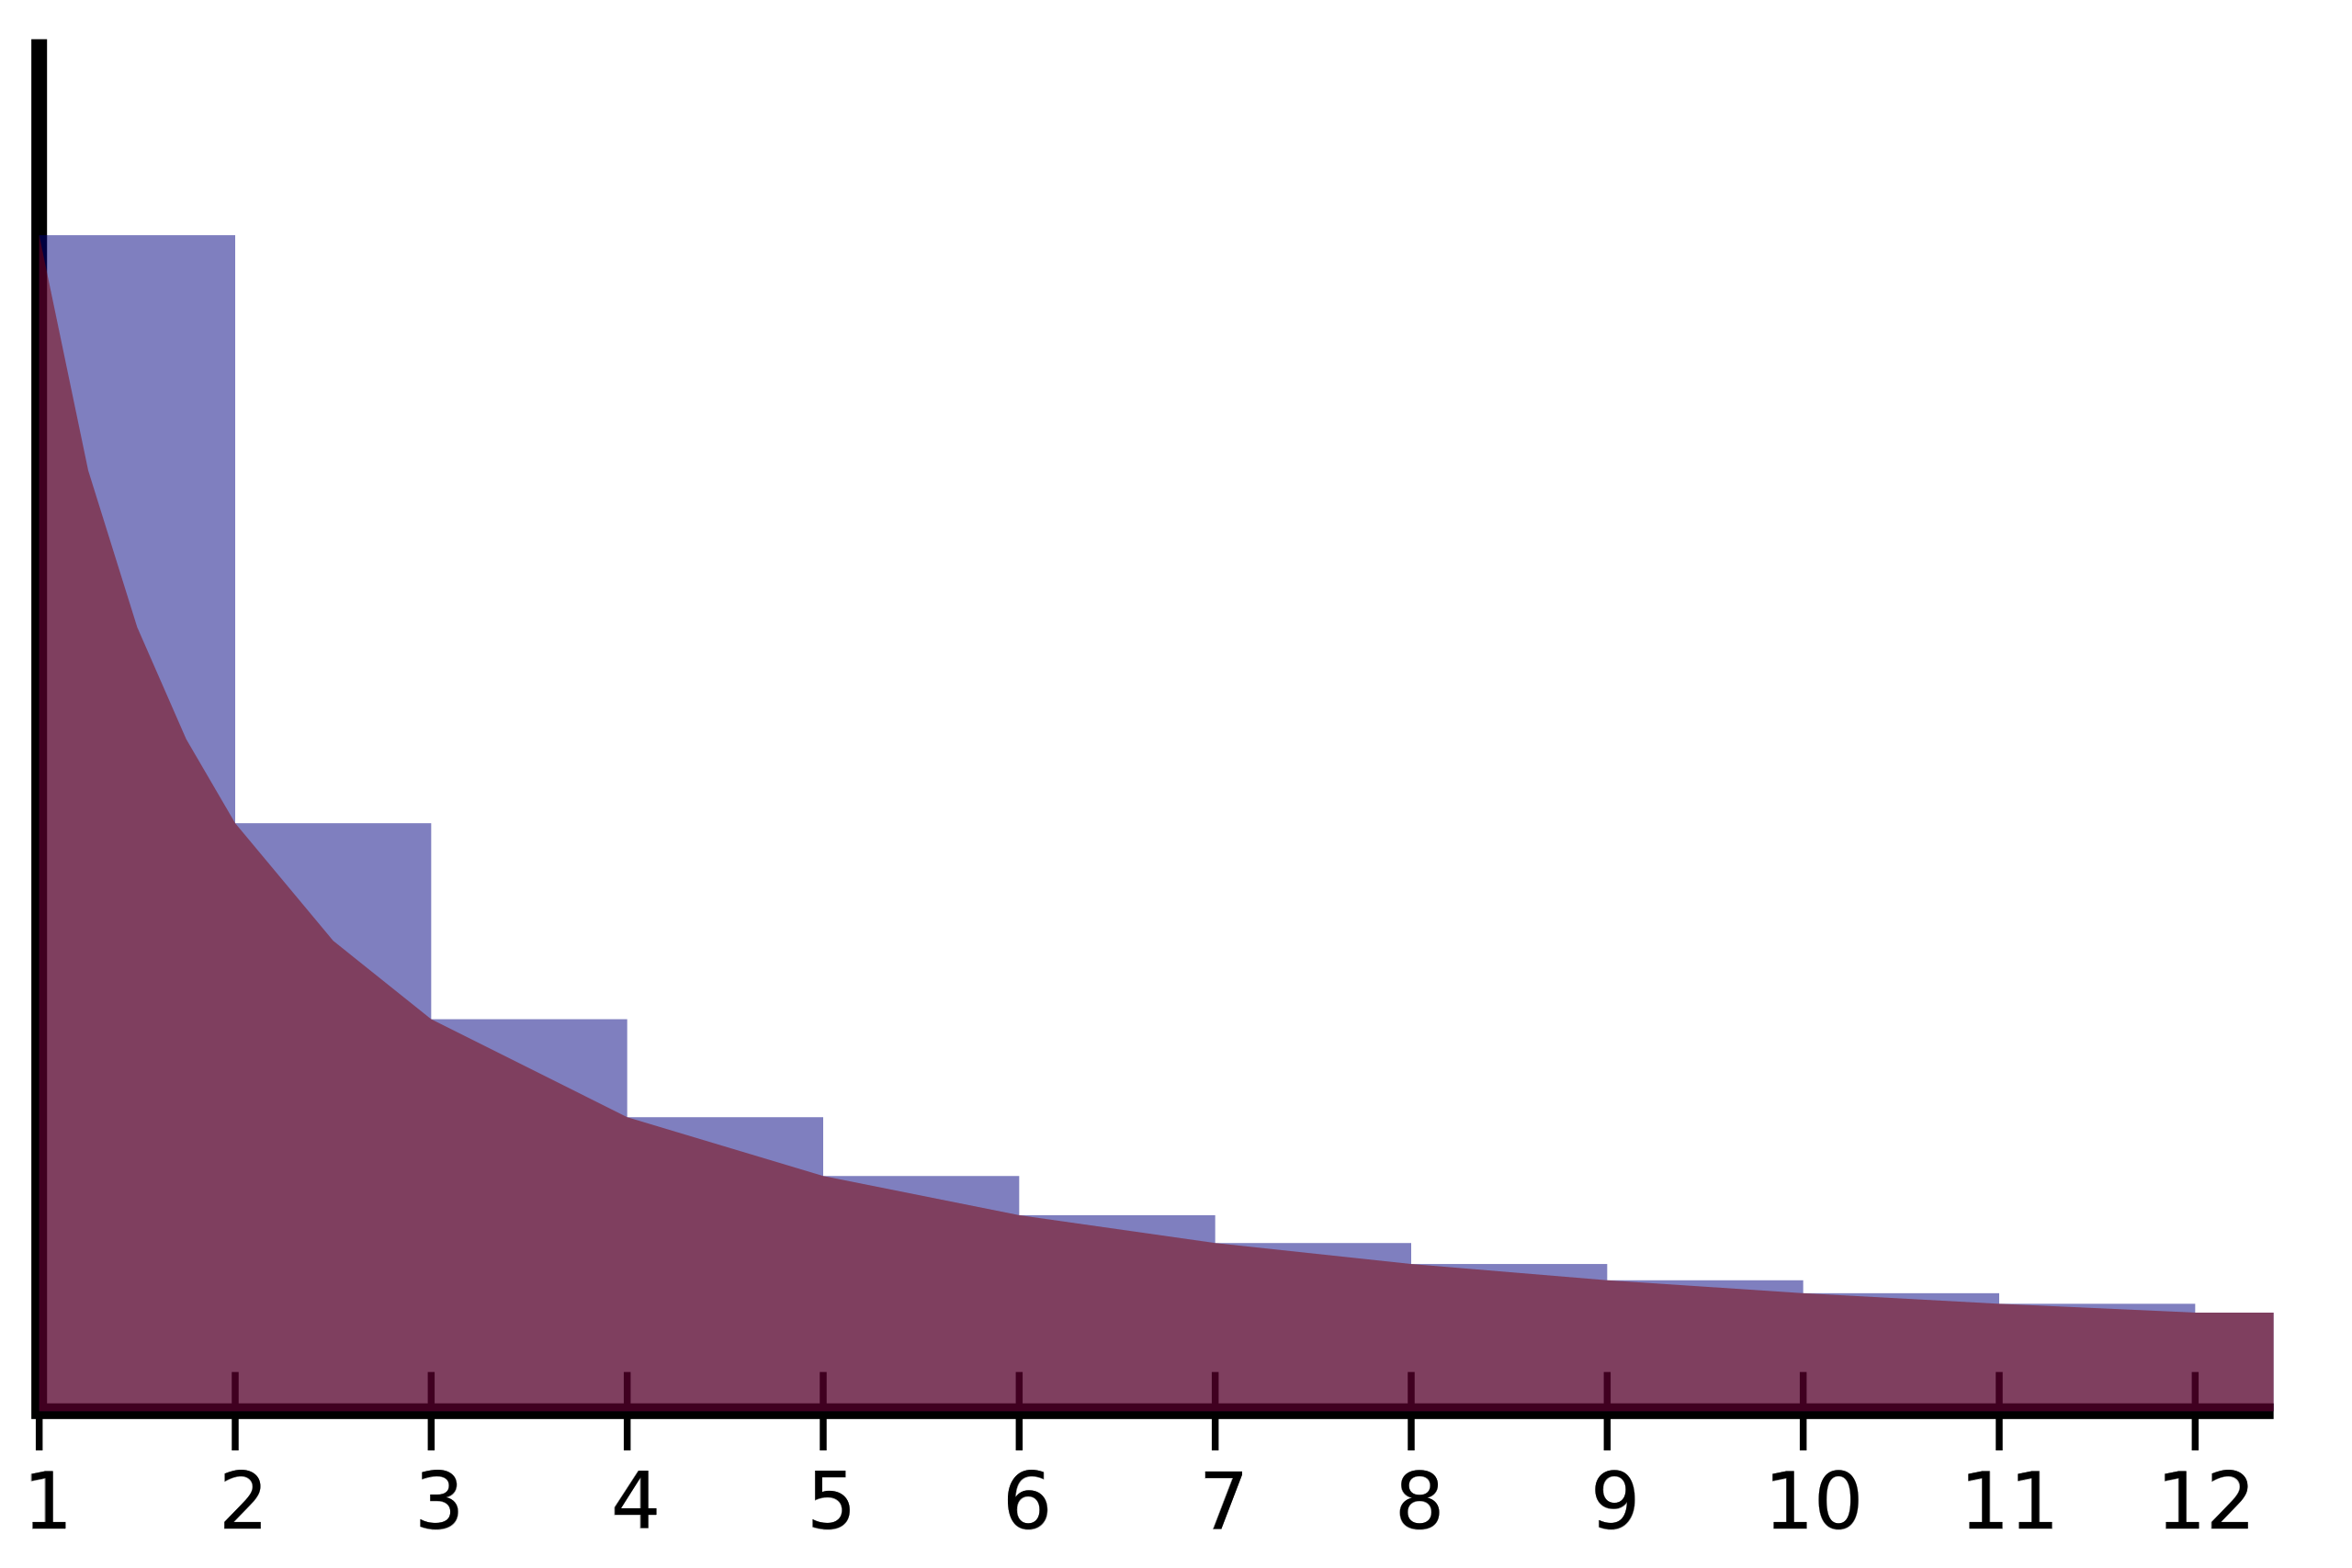
\includegraphics[scale=0.05]{img/em.png}
        \end{center}
    \end{frame}

    \begin{frame}
        \frametitle{Quiz}
        \begin{center}
            Both transcendence and irrationality are unknown.
        \end{center}
    \end{frame}

    \begin{frame}
        \frametitle{Quiz}
        \begin{center}
            \[\lambda,\] 
            Conway's constant or $1.3035772690\ldots$ \\
        \end{center}
    \end{frame}

     \begin{frame}
        \frametitle{Quiz}
        \begin{center}
 
            Look and say sequence \[(a_n) = 1, 11, 21, 1211, 111221, 312211, \ldots\]

            \[\lambda = \lim\limits_{n \to \infty} \frac{\text{length}(a_{n+1})}{\text{length}(a_{n})}\]
        \end{center}
    \end{frame}

    \begin{frame}
        \frametitle{Quiz}
        \begin{center}
            Algebraic. Minimal polynomial has degree 71!
            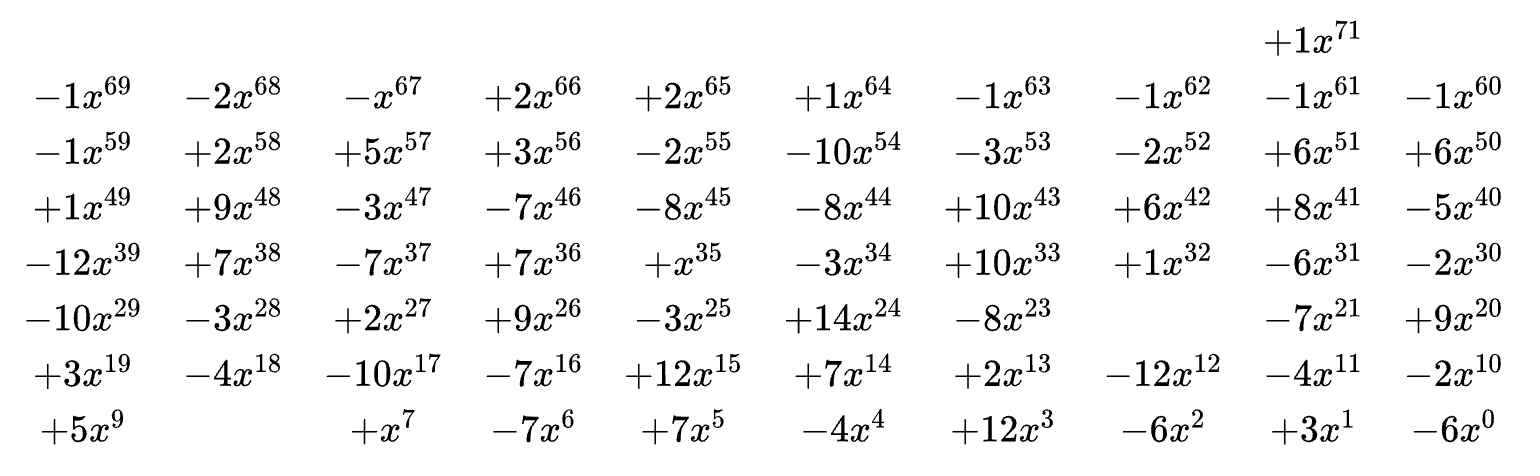
\includegraphics[scale=0.35]{img/mp.png}
        \end{center}
    \end{frame}

    \begin{frame}
        \frametitle{Algebraic Independence}
        \begin{center}
            \begin{mybox}
                \textbf{Definition:} Let $L/K$ be a field extension. Then $S = \{s_1, \ldots, s_t\} \subseteq L$ is \vocab{algebraically independent} over $K$ if for all $f \in K[x_1, \ldots, x_t]$, $f(s_1, \ldots, s_t) = 0 \implies f = 0$.
            \end{mybox}
            Stronger than linear independence. $\{\pi\}$ is algebraically independent over $\Q$.\par
        \end{center}
    \end{frame}

    \begin{frame}
        \frametitle{Transcendence Basis}
        \begin{center}
            \begin{mybox}
                \textbf{Definition:} Let $L/K$ be a field extension. The maximal algebraically independent subset of $L$ is called a \vocab{transcendence basis} of $L/K$. It's cardinality is called the \vocab{transcendence degree} denoted $\trdeg(L/K)$.
            \end{mybox}
            All transcendence bases have the same size. 
            $\trdeg(M/K) = \trdeg(M/L) + \trdeg(L/K)$. \\
            $\trdeg(\Q(\sqrt{2})/\Q) = 0$ \\ $\trdeg(\Q(\pi)/\Q) = 1$ \\ $\trdeg(\R/\Q) = 2^{\aleph_0}$
        \end{center}
    \end{frame}

    \begin{frame}
        \frametitle{Lindemann-Weierstrass Theorem}
        \begin{center}
            \begin{mybox}
                \textbf{Lindemann-Weierstrass Theorem:} If $\alpha_1, \ldots, \alpha_n \in \A$, then $\{e^{\alpha_1}, \ldots, e^{\alpha_n}\}$ is $\A$-linearly independent.
            \end{mybox}       
            equivalently, $\trdeg(\Q(e^{\alpha_1}, \ldots, e^{\alpha_n})/\Q) = n$.
        \end{center}
    \end{frame}

    \begin{frame}
    \frametitle{Auxiliary Functions}
    \begin{center}
    Proof uses a cleverly constructed auxiliary function with nice properties (many zeroes or zeroes with high multiplicity) to form a contradiction. In Liouville's Approximation theorem, the auxiliary function was the minimal polynomial.\par

    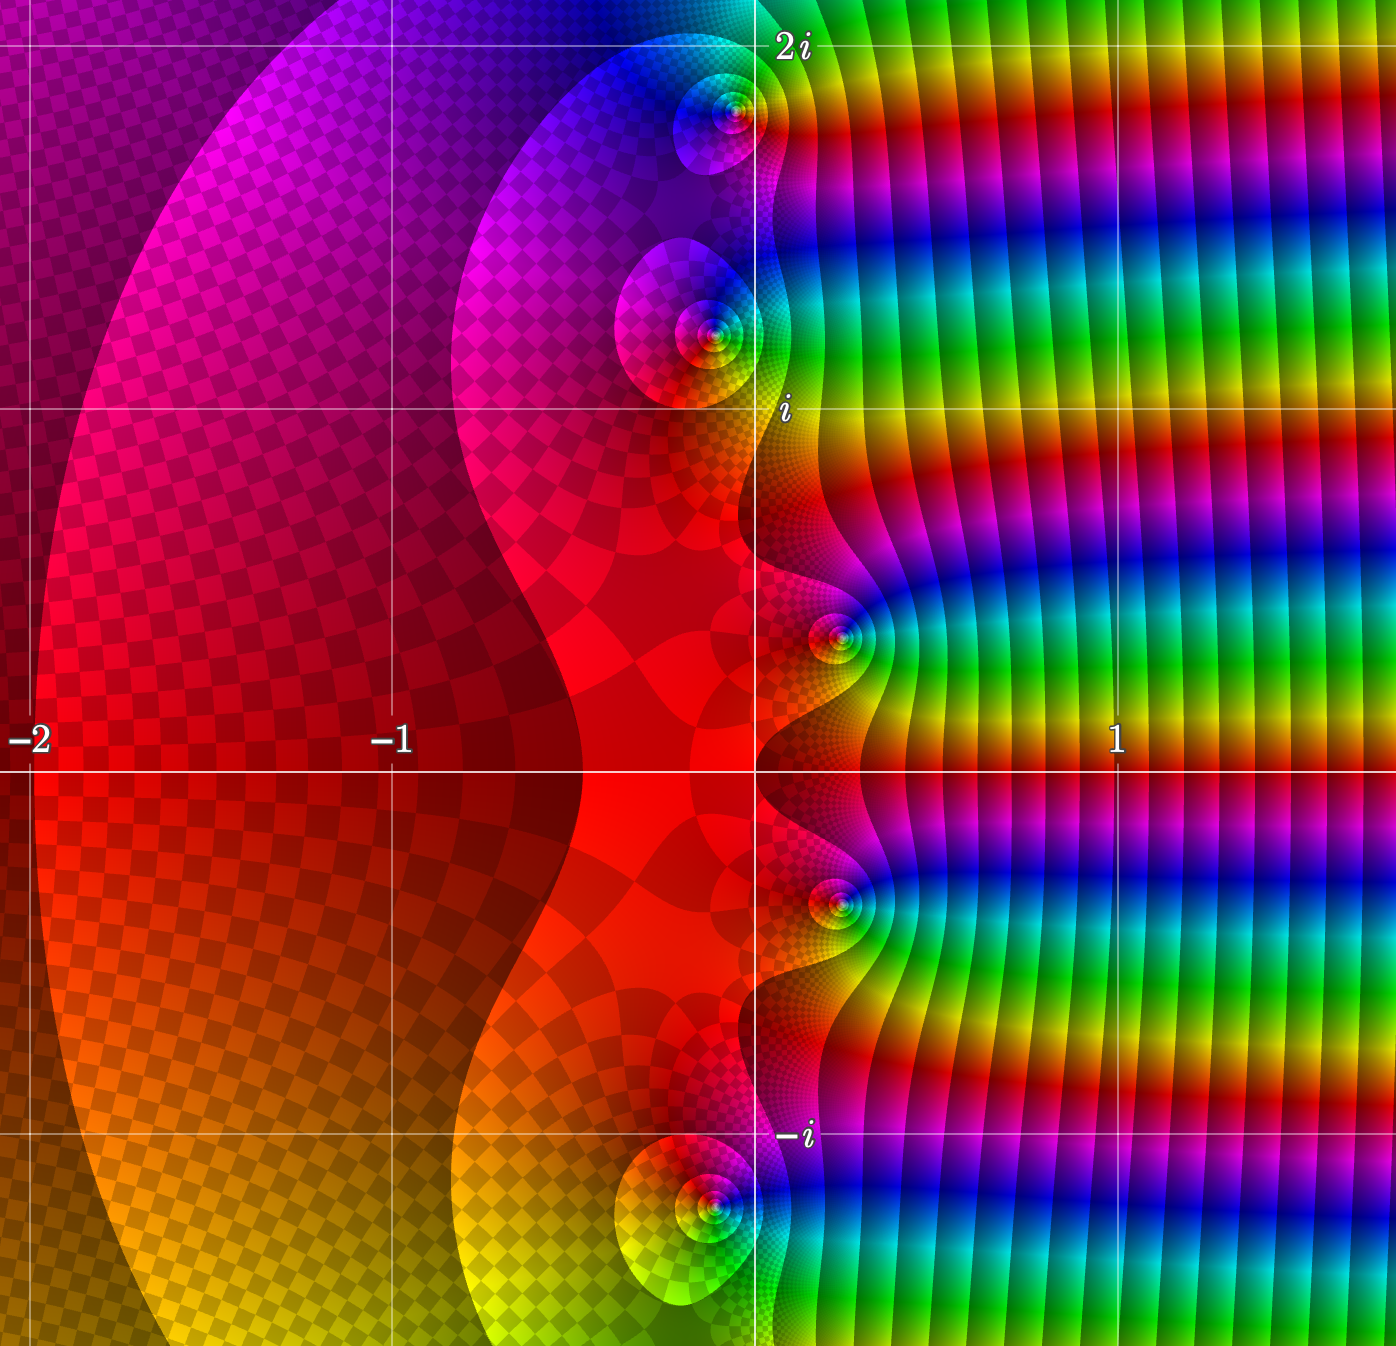
\includegraphics[scale=0.1]{img/domain.png}\par
    \href{https://samuelj.li/complex-function-plotter/}{Gelfond's Auxiliary Function}
    \end{center}
    \end{frame}

    \begin{frame}
    \frametitle{Auxiliary Functions}
    \begin{center}
        Let the function
        \[P(x,y) = \sum\limits_{m=0}^{D-1}\sum\limits_{n=1}^{D-1}a_{m,n}{x}^{m}y^{n} \in \Z[x,y]\]
        Lindemann-Weierstrass theorem uses the auxiliary function $F(z) = P(e^{z}, e^{iz})$
    \end{center}
    \end{frame}

    \begin{frame}
        \frametitle{Corollary}
        \begin{center}
            \begin{mybox}
                \textbf{Lindemann-Weierstrass Theorem:} If $\alpha_1, \ldots, \alpha_n \in \A$, then $\{e^{\alpha_1}, \ldots, e^{\alpha_n}\}$ is $\A$-linearly independent.
            \end{mybox}       
            Set $\alpha_1 = 0, \alpha_2 = 1$. Shows $e$ is transcendental. \\
            Set $\alpha_1 = 0, \alpha_2 = \alpha_2$. Shows $e^{\alpha_2}$ is transcendental. \\
            AFSOC, set $\alpha_1 = 0, \alpha_2 = \pi i$. Shows $\pi i$ is transcendental; we know $i \in \A$ so $\pi \notin \A$. 
        \end{center}
    \end{frame}

    \begin{frame}
        \frametitle{Gelfond-Schneider Theorem}
        \begin{center}
            \begin{mybox}
                \textbf{Gelfond-Schneider Theorem:} If $\alpha, \beta \in \A$, $\alpha \neq 0, 1$, $\beta \notin \Q$, then any value of ${\alpha}^{\beta}$ is transcendental.
            \end{mybox}       
            Answers Hilbert's Seventh Problem.
            \[2^{\log_2(21441)} = 21441\] so $\log_2(21441)$ is either transcendental or rational.\par
            $e^{\pi} = {\left(e^{\pi i}\right)}^{-i} = {(-1)}^{-i}$ is transcendental.
        \end{center}
    \end{frame}

    \begin{frame}
        \frametitle{Auxiliary Functions Used}
        \begin{center}
        Let the function
        \[P(x,y) = \sum\limits_{m=0}^{D-1}\sum\limits_{n=1}^{D-1}a_{m,n}{x}^{m}y^{n} \in \Z[x,y]\]

        Gelfond used Taylor series of $F(z) = P(e^{z}, e^{\beta z})$. Has zeroes of high multiplicity.\par

        Schneider used $F(z) = P(e^{z}, e^{\log(\alpha)z})$. Has many zeroes of multiplicity one.\par
        \end{center}
    \end{frame}

    \begin{frame}
        \frametitle{Baker's Theorem}
        \begin{center}
        \begin{mybox}
            \textbf{Baker's Theorem:} Let nonzero $\alpha_1, \ldots, \alpha_n \in \A$. Then, if $2\pi i, \log(\alpha_1), \ldots, \log(\alpha_{n})$ are $\Q$-linearly independent, they are also $\A$-linearly independent.
        \end{mybox}
        Alan Baker later showed it the statement is still true without $2 \pi i$. Auxiliary function was \[F(z_1, \ldots, z_n) = \] \[\sum\limits_{\lambda_1 = 0}^{L}\sum\limits_{\lambda_2=0}^{L} \cdots \sum\limits_{\lambda_n = 0}^{L}p(\lambda_1, \lambda_2, \ldots, \lambda_n)\alpha_1^{(\lambda_1 + \lambda_n\beta)z_1}\cdots \alpha_{n-1}^{(\lambda_{n-1}+\lambda_{n}\beta)z_{n-1}}\]
        \end{center}
    \end{frame}

    \begin{frame}
        \frametitle{Corollary}
        Baker's theorem generalizes the Lindemann-Weierstrass and Gelfond-Schneider theorems. For $a_1, \ldots, a_n \in \A$ not $0$ or $1$, and $\beta_1, \ldots, \beta_n \in \A \setminus \Q$ and $\Q$-linearly independent, ${a_1}^{\beta_1}\cdots {a_n}^{\beta_n}$ is transcendental.
    \end{frame}

    \begin{frame}
        \frametitle{Schanuel's Conjecture}
        \begin{center}
        \begin{mybox}
            \textbf{Schanuel's Conjecture:} If $z_1, \ldots, z_n$ be $\Q$-linearly independent, $\trdeg(\Q(z_1, \ldots, z_n, e^{z_1}, \ldots, e^{z_n})/\Q) \geq n$. 
        \end{mybox}
        No progress for 60 years. Setting $z_1 = 1, z_2 = \pi i$ shows algebraic independence of $e$ and $\pi$. Setting $z_1 = 1$, $z_2 = e$ shows transcendence of $e^{e}$.
        Setting $z_1 = \log \log \pi, z_2 = 1 + \log \log \pi, z_3 = \log \pi, z_4 = e \log \pi, z_5 = i \pi$, one can show $\pi^{e}$ is transcendental. 
        \end{center}
    \end{frame}
    \begin{frame}
        \frametitle{References}
        \begin{thebibliography}{99} % Beamer does not support BibTeX so references must be inserted manually as below, you may need to use multiple columns and/or reduce the font size further if you have many references
		\footnotesize % Reduce the font size in the bibliography
	
		\bibitem[Niven, 1956]{p1}
			 Ivan Niven
             \newblock{Irrational Numbers}

        \bibitem[Conway, 1996]{p2}
            John Conway
            \newblock{The Look and Say Sequence}

		\bibitem[Burger, 2004]{p3}
            Edward Burger 
            \newblock{Making Transcendence Transparent}

            \bibitem[Wolfram MathWorld]{p4}
            Wolfram MathWorld
            \newblock{Schanuel's Conjecture}
        
            \bibitem[Gelfond, 1959]{p5}
            Alexander Gelfond
            \newblock{Transcendental and Algebraic Numbers}

        \bibitem[Baker, 1975]{p6}
            Alan Baker 
            \newblock{Transcendental Number Theory}

        \bibitem[Soundararajan, 2011]{p7}
            Kannan Soundararajan
            \newblock{Transcendental Number Theory}

	\end{thebibliography} 
    \end{frame}

    \begin{frame}
        \begin{center}
            {\bfseries\huge\gradientRGB{Thank You!}{20,220,100}{50,200,200}} \par
            Questions?
        \end{center}
    \end{frame}

\end{document}
